\documentclass[tikz,border=10pt]{standalone}
\usepackage{amsmath}
\usetikzlibrary{decorations.pathmorphing,arrows.meta}

\begin{document}
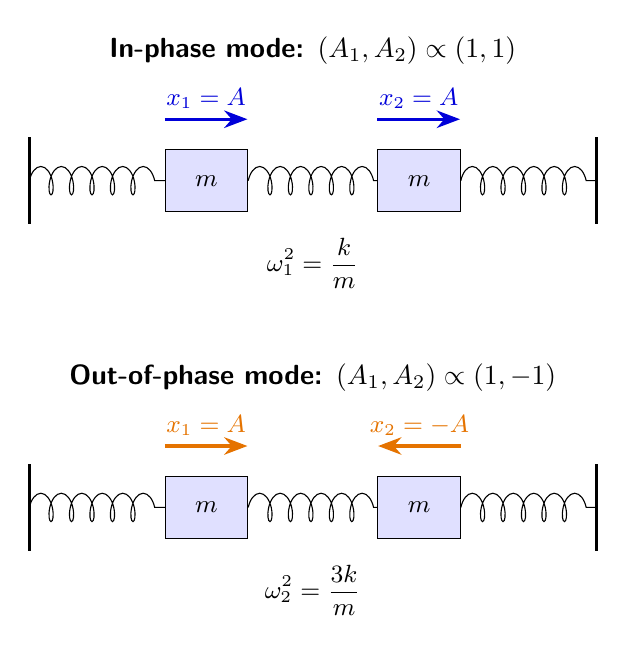
\begin{tikzpicture}[
  >=Stealth,
  font=\sffamily\small,
  block/.style={draw,fill=blue!12,minimum width=1.05cm,minimum height=.78cm},
  spring/.style={decorate,decoration={coil,aspect=.45,segment length=2.6mm,amplitude=1.8mm}},
  move/.style={->,very thick}
]
  % In-phase mode.
  \begin{scope}[yshift=4.15cm]
    \node[font=\sffamily\bfseries] at (3.6,1.65)
      {In-phase mode: $(A_1,A_2)\propto(1,1)$};
    \draw[very thick] (0,-.55)--(0,.55) (7.2,-.55)--(7.2,.55);
    \draw[spring] (0,0)--(1.75,0);
    \node[block] at (2.25,0) {$m$};
    \draw[spring] (2.78,0)--(4.42,0);
    \node[block] at (4.95,0) {$m$};
    \draw[spring] (5.48,0)--(7.2,0);
    \draw[move,blue!85!black] (1.72,.78)--(2.77,.78)
      node[midway,above] {$x_1=A$};
    \draw[move,blue!85!black] (4.42,.78)--(5.47,.78)
      node[midway,above] {$x_2=A$};
    \node at (3.6,-1.05) {$\displaystyle \omega_1^2=\frac{k}{m}$};
  \end{scope}

  % Out-of-phase mode.
  \begin{scope}
    \node[font=\sffamily\bfseries] at (3.6,1.65)
      {Out-of-phase mode: $(A_1,A_2)\propto(1,-1)$};
    \draw[very thick] (0,-.55)--(0,.55) (7.2,-.55)--(7.2,.55);
    \draw[spring] (0,0)--(1.75,0);
    \node[block] at (2.25,0) {$m$};
    \draw[spring] (2.78,0)--(4.42,0);
    \node[block] at (4.95,0) {$m$};
    \draw[spring] (5.48,0)--(7.2,0);
    \draw[move,orange!90!black] (1.72,.78)--(2.77,.78)
      node[midway,above] {$x_1=A$};
    \draw[move,orange!90!black] (5.48,.78)--(4.43,.78)
      node[midway,above] {$x_2=-A$};
    \node at (3.6,-1.05) {$\displaystyle \omega_2^2=\frac{3k}{m}$};
  \end{scope}
\end{tikzpicture}
\end{document}
